\anexo{Resultados de la encuesta}\label{anexo:encuesta}

\begin{figure}[H]
    \centering
    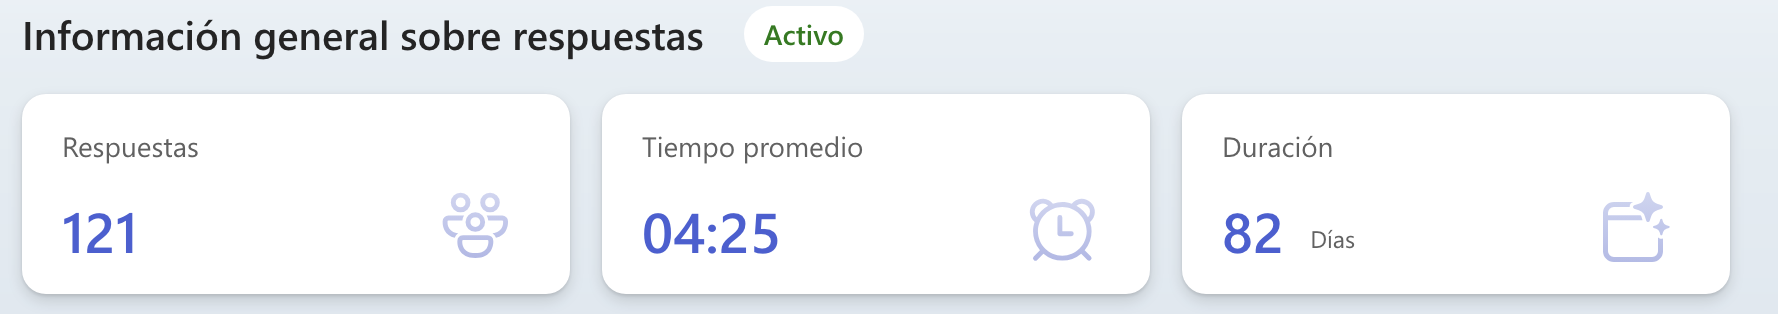
\includegraphics[width=0.6\textwidth]{Imagenes/Encuesta/Datos_Generales}
    \caption[Datos generales de la encuesta.]{Datos generales de la encuesta, con 121 respuestas válidas con un tiempo promedio de respuesta de 4 minutos 25 segundos.
    \newline\footnotesize\textit{Fuente: Elaboración propia.}}
    \label{fig:encuesta_general}
\end{figure}

\begin{figure}[H]
    \centering
    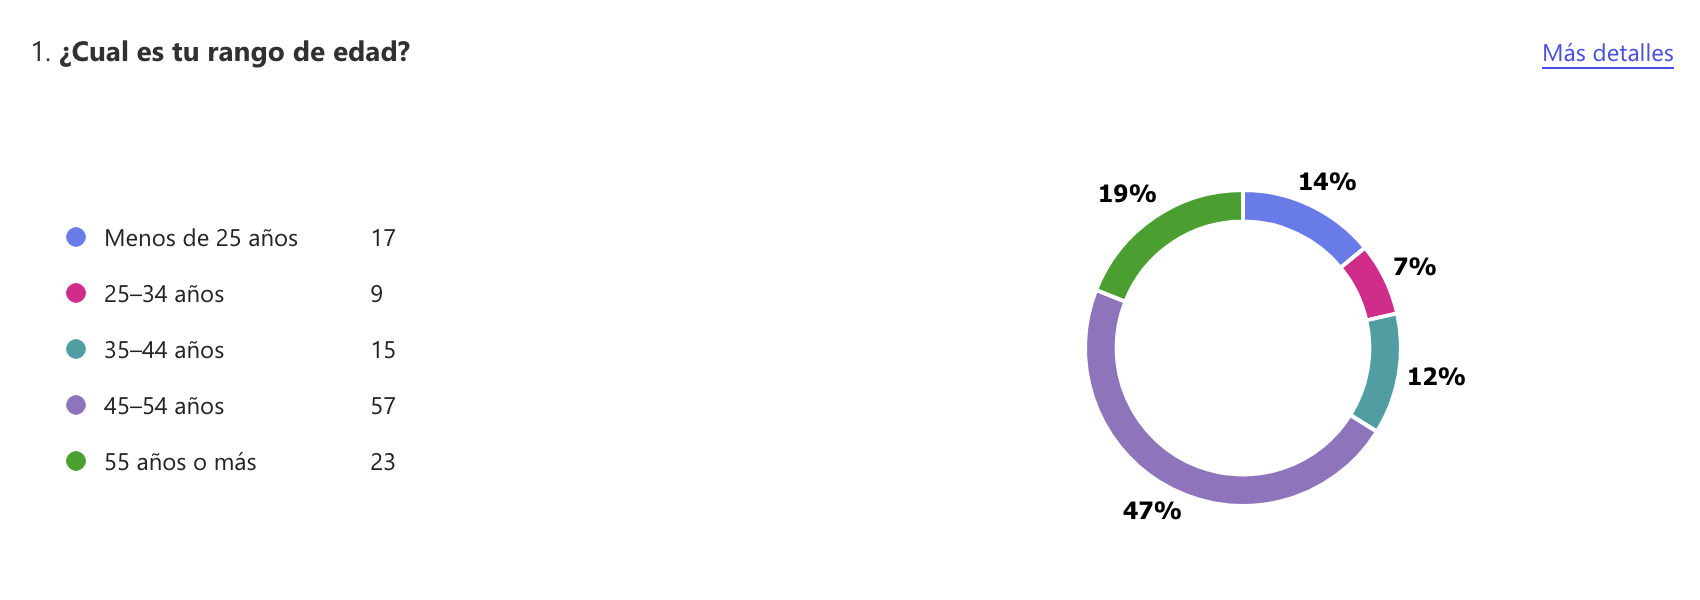
\includegraphics[width=0.85\textwidth]{Imagenes/Encuesta/Encuesta_Q1}
    \caption[Distribución por rango etario de los encuestados.]{Distribución por rango etario de los encuestados. El 47\,\% tiene entre 45 y 54~años y un 19\,\% adicional tiene 55~años o más.
    \newline\footnotesize\textit{Fuente: Elaboración propia.}}
    \label{fig:encuesta_q1}
\end{figure}

\begin{figure}[H]
    \centering
    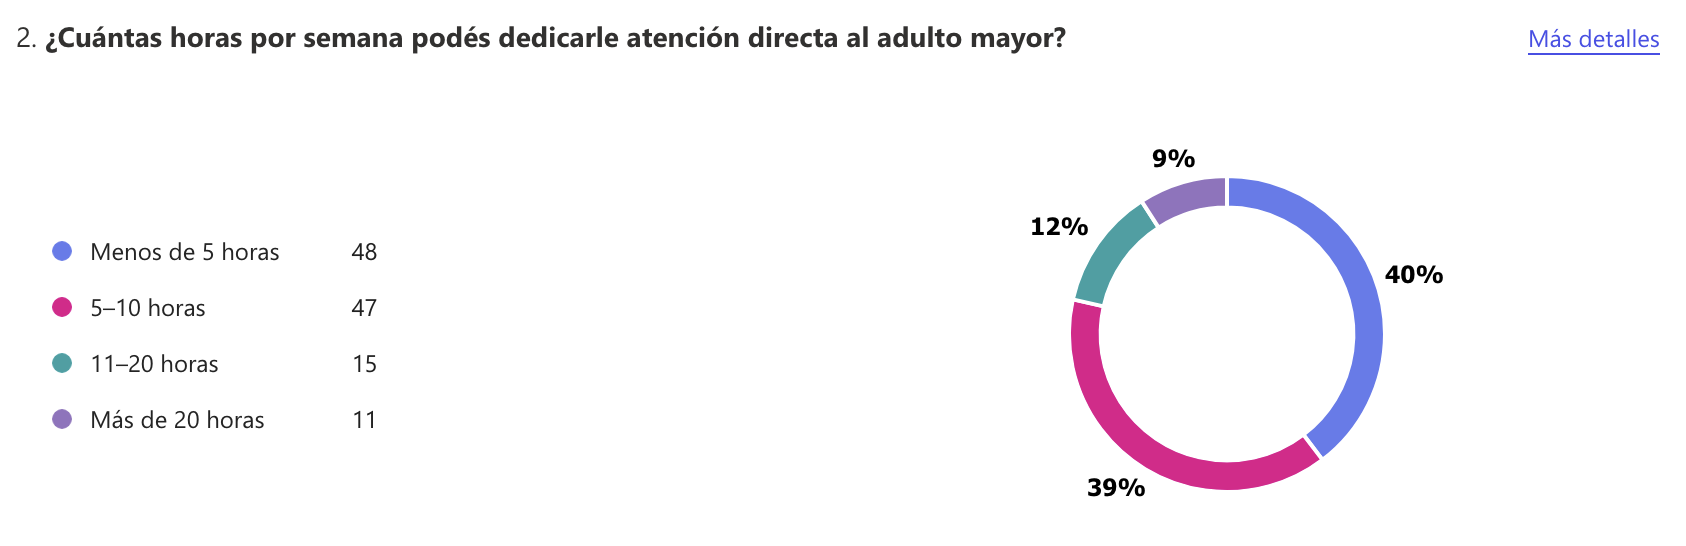
\includegraphics[width=0.85\textwidth]{Imagenes/Encuesta/Encuesta_Q2}
    \caption[Horas semanales de atención directa al adulto mayor.]{Horas semanales de atención directa al adulto mayor. El 79\,\% dedica menos de 10~horas semanales de atención directa.
    \newline\footnotesize\textit{Fuente: Elaboración propia.}}
    \label{fig:encuesta_q2}
\end{figure}

\begin{figure}[H]
    \centering
    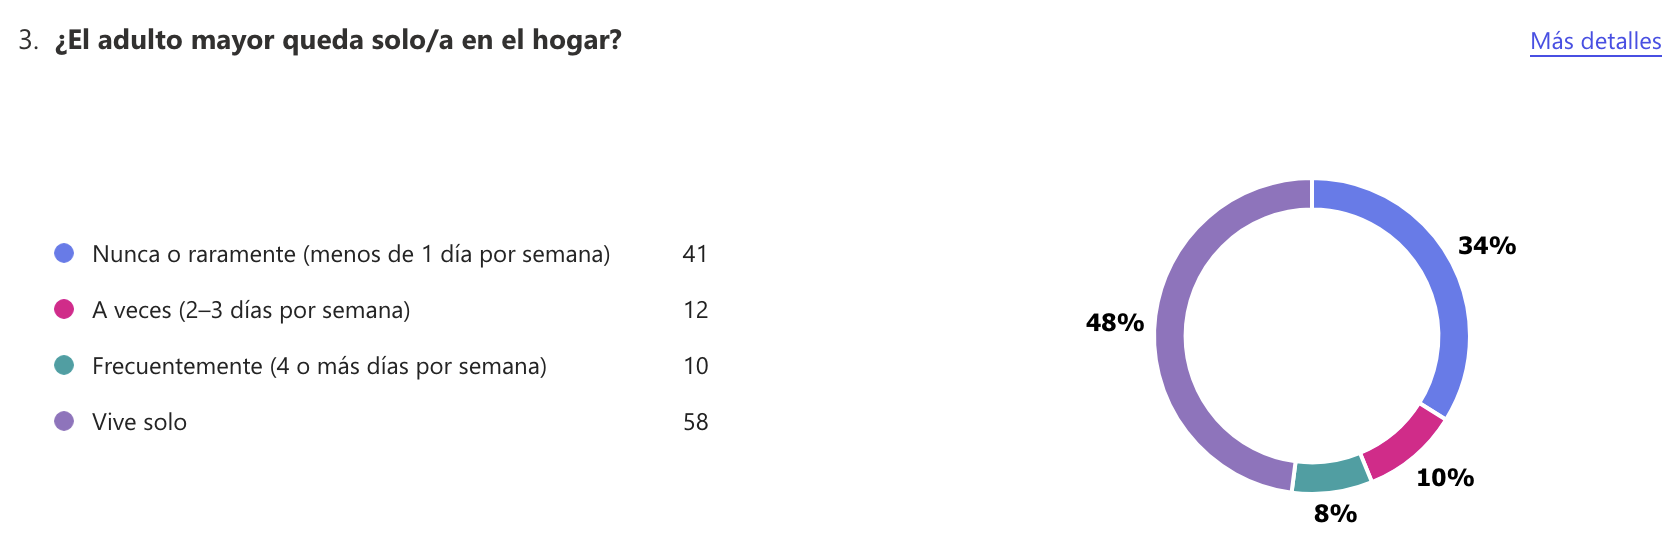
\includegraphics[width=0.85\textwidth]{Imagenes/Encuesta/Encuesta_Q3}
    \caption[Frecuencia con la que el adulto mayor queda solo en el hogar.]{Frecuencia con la que el adulto mayor queda solo en el hogar. El 48\,\% vive solo de forma permanente y un 18\,\% adicional queda solo con cierta frecuencia.
    \newline\footnotesize\textit{Fuente: Elaboración propia.}}
    \label{fig:encuesta_q3}
\end{figure}

\begin{figure}[H]
    \centering
    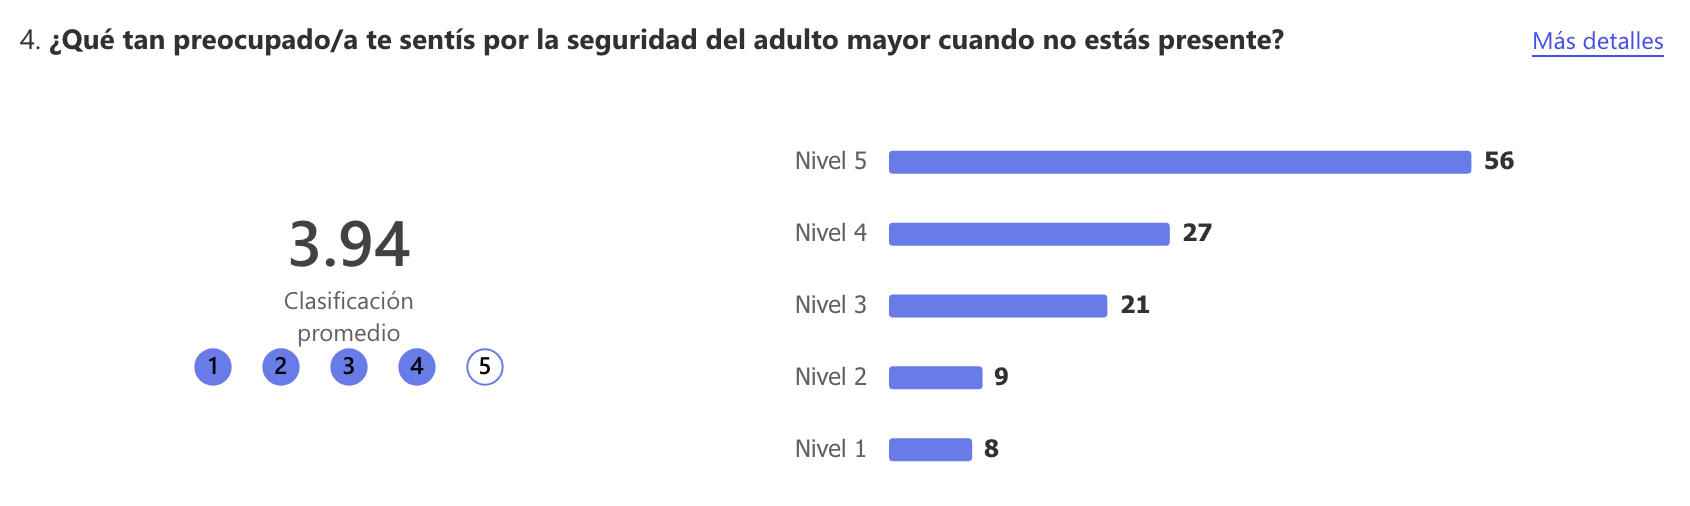
\includegraphics[width=0.85\textwidth]{Imagenes/Encuesta/Encuesta_Q4}
    \caption[Nivel de preocupación por la seguridad del adulto mayor sin supervisión.]{Nivel de preocupación por la seguridad del adulto mayor sin supervisión (escala 1--5). El 69\,\% marcó los valores más altos de la escala.
    \newline\footnotesize\textit{Fuente: Elaboración propia.}}
    \label{fig:encuesta_q4}
\end{figure}

\begin{figure}[H]
    \centering
    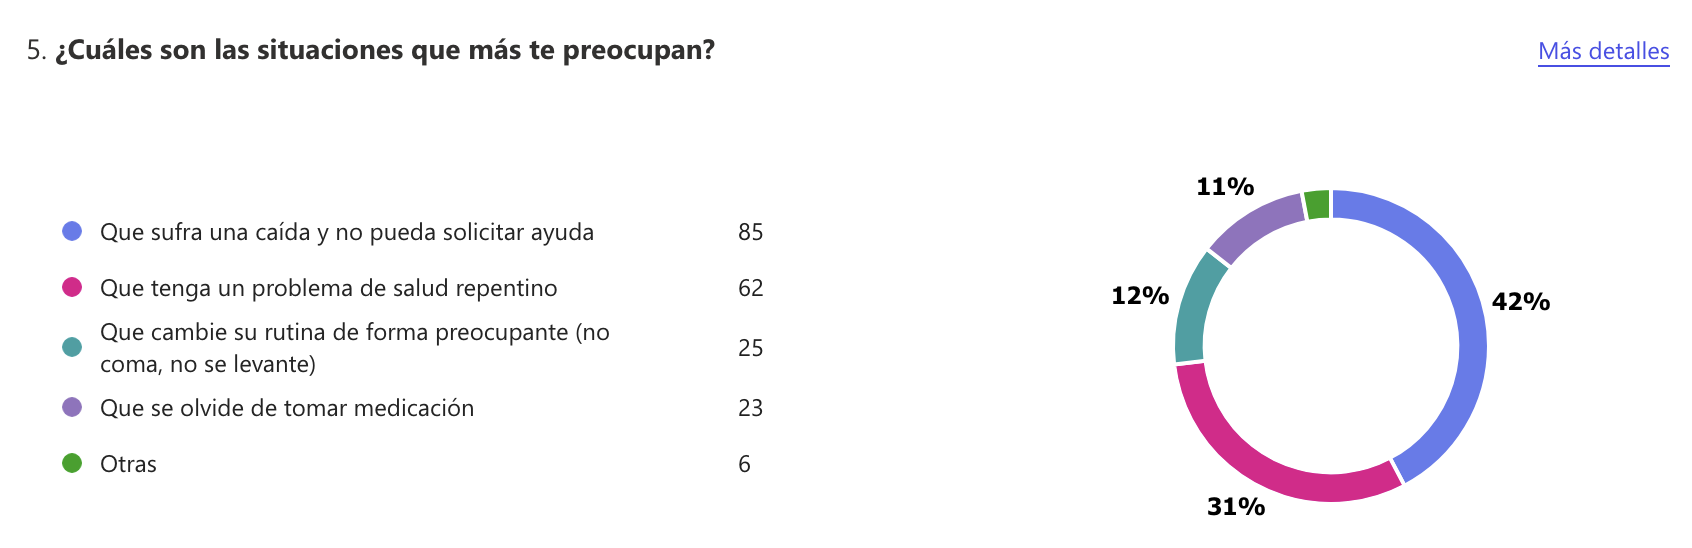
\includegraphics[width=0.85\textwidth]{Imagenes/Encuesta/Encuesta_Q5}
    \caption[Situaciones que más preocupan a los cuidadores familiares.]{Situaciones que más preocupan a los cuidadores familiares. La caída sin posibilidad de pedir ayuda encabeza el ranking, mencionada en el 70\,\% de las respuestas.
    \newline\footnotesize\textit{Fuente: Elaboración propia.}}
    \label{fig:encuesta_q5}
\end{figure}

\begin{figure}[H]
    \centering
    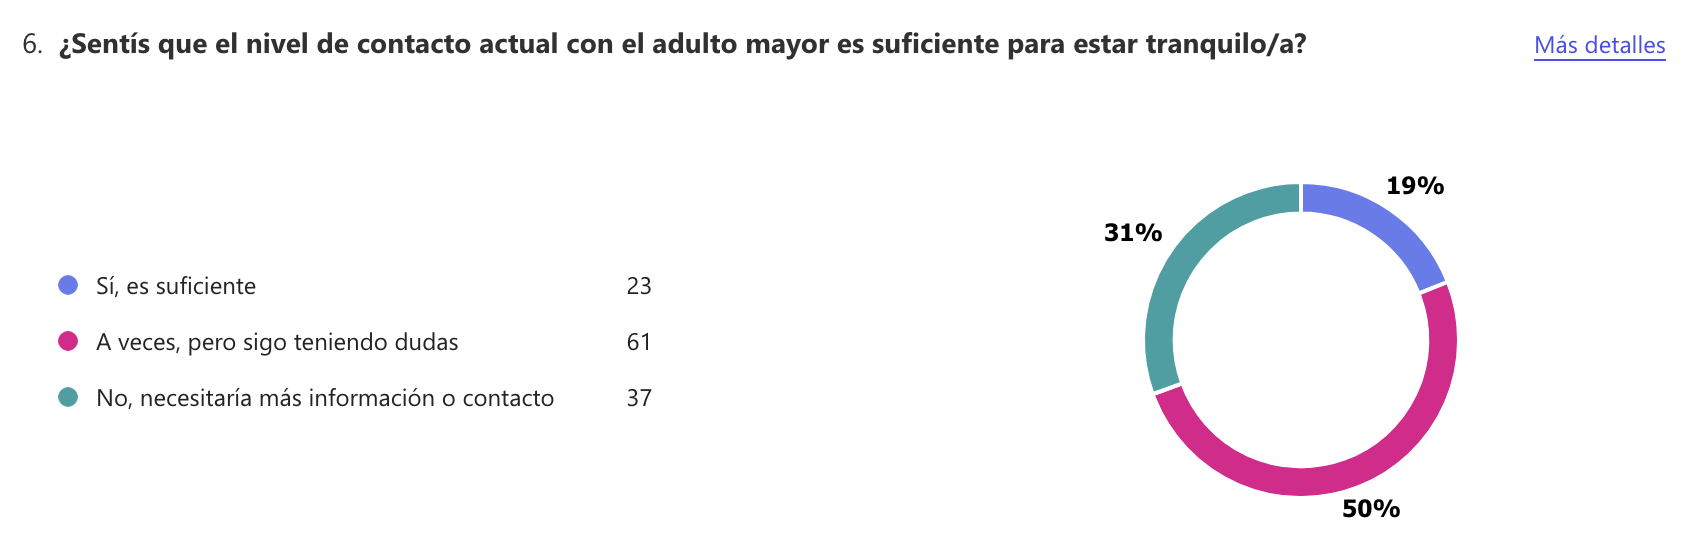
\includegraphics[width=0.85\textwidth]{Imagenes/Encuesta/Encuesta_Q6}
    \caption[Percepción sobre la suficiencia del contacto actual con el adulto mayor.]{Percepción sobre la suficiencia del contacto actual con el adulto mayor. Solo el 19\,\% lo considera suficiente, el 50\,\% todavía tiene dudas y el 31\,\% necesitaría más información o más contacto.
    \newline\footnotesize\textit{Fuente: Elaboración propia.}}
    \label{fig:encuesta_q6}
\end{figure}

\begin{figure}[H]
    \centering
    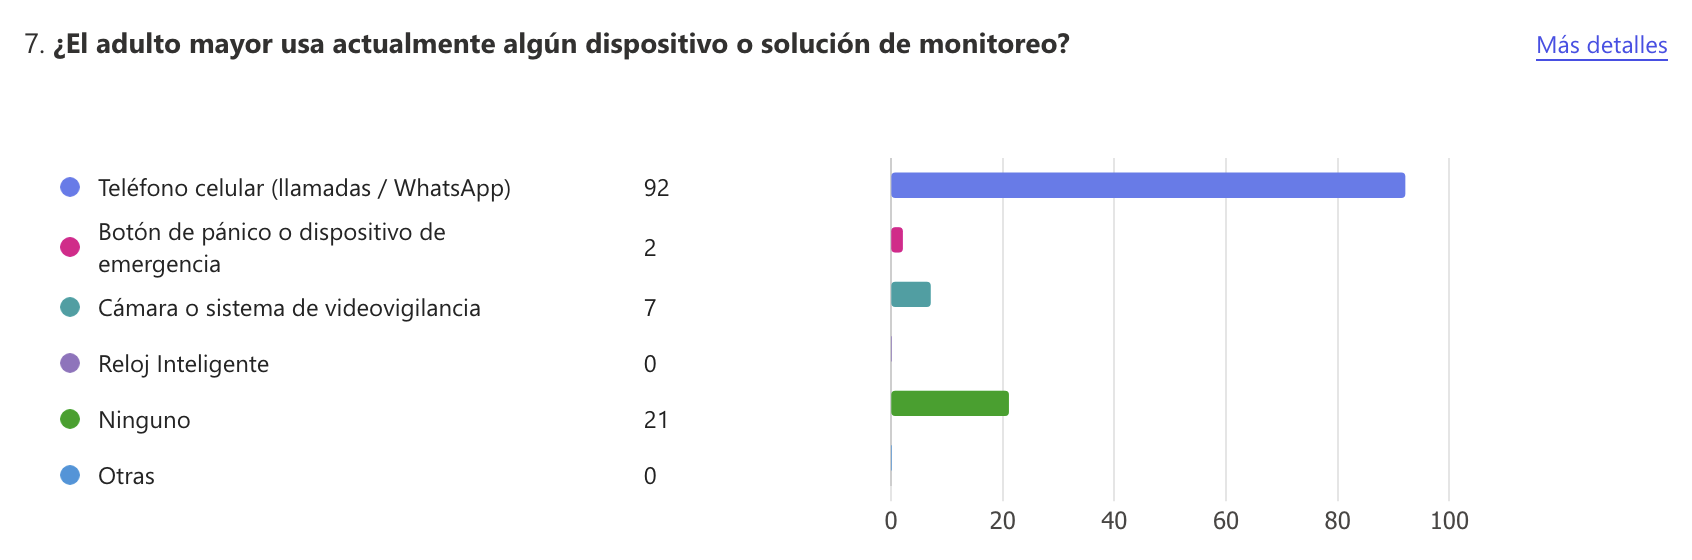
\includegraphics[width=0.85\textwidth]{Imagenes/Encuesta/Encuesta_Q7}
    \caption[Soluciones de monitoreo utilizadas actualmente por los cuidadores.]{Soluciones de monitoreo utilizadas actualmente por los cuidadores. El 76\,\% usa el teléfono celular y solo el 7\,\% utiliza videovigilancia o botón de pánico.
    \newline\footnotesize\textit{Fuente: Elaboración propia.}}
    \label{fig:encuesta_q7}
\end{figure}

\begin{figure}[H]
    \centering
    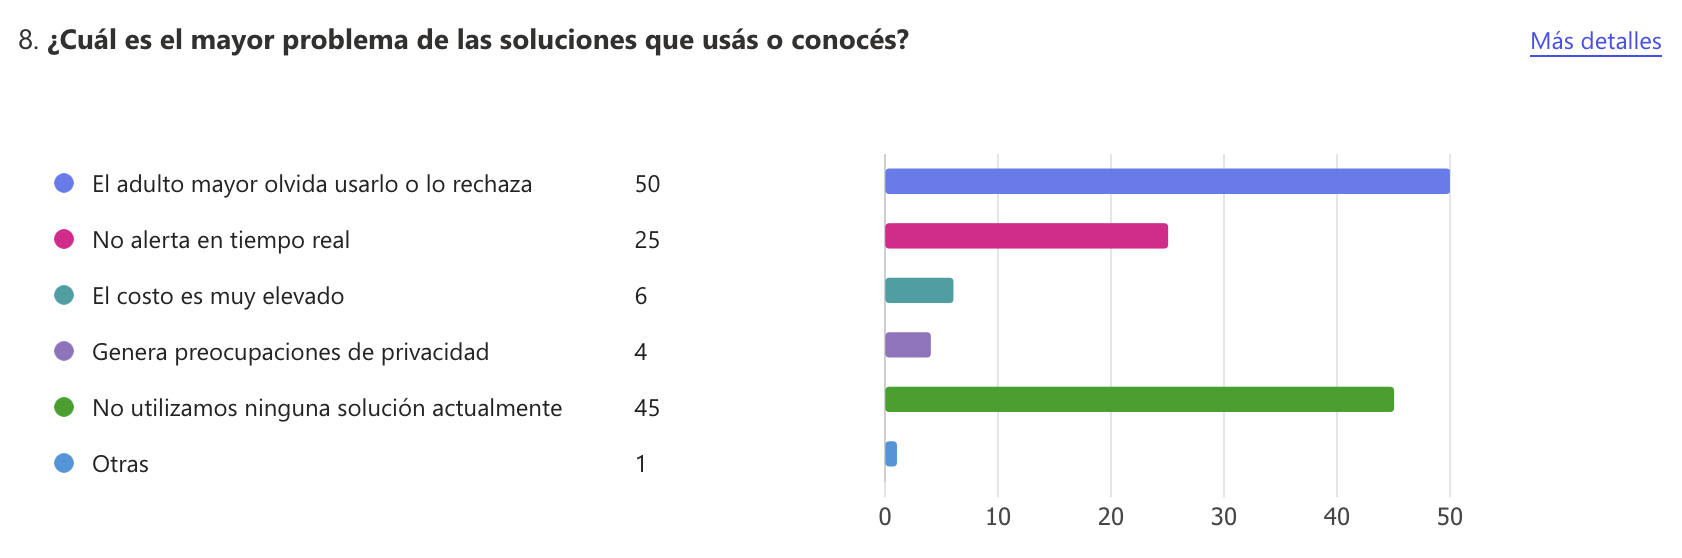
\includegraphics[width=0.85\textwidth]{Imagenes/Encuesta/Encuesta_Q8}
    \caption[Principal problema de las soluciones de monitoreo existentes.]{Principal problema de las soluciones de monitoreo existentes. El 41\,\% reporta que el adulto mayor olvida o rechaza el dispositivo, y un 37\,\% no usa ninguna solución.
    \newline\footnotesize\textit{Fuente: Elaboración propia.}}
    \label{fig:encuesta_q8}
\end{figure}

\begin{figure}[H]
    \centering
    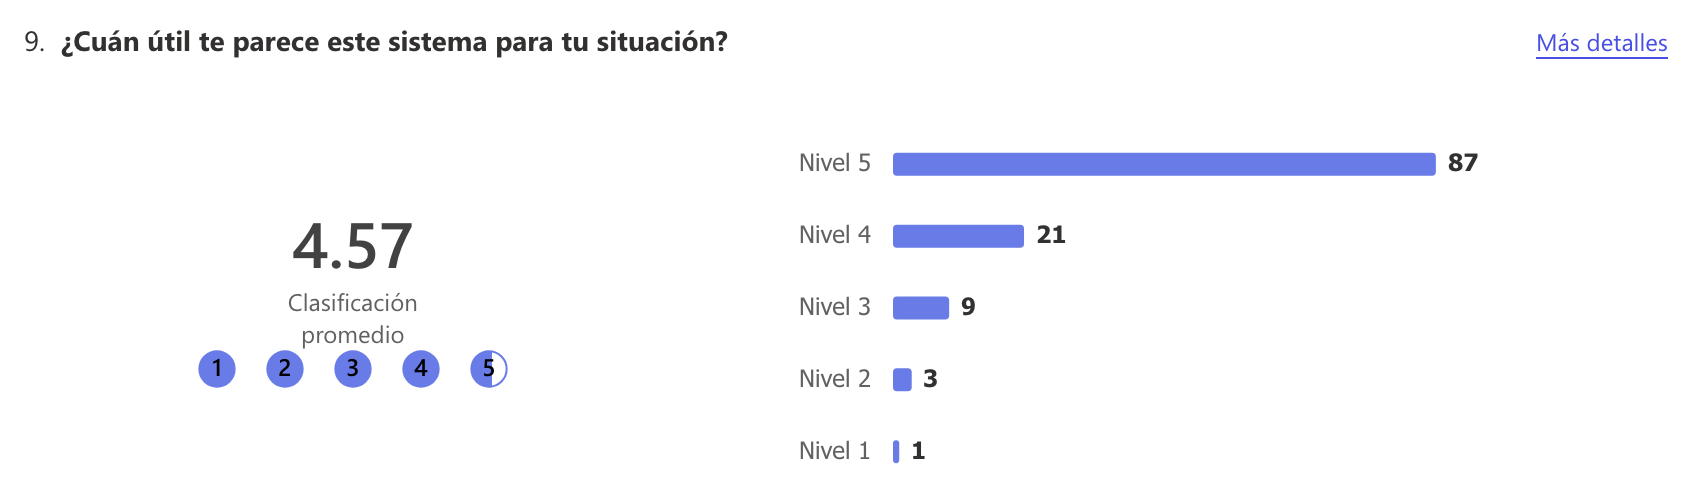
\includegraphics[width=0.85\textwidth]{Imagenes/Encuesta/Encuesta_Q9}
    \caption[Valoración de utilidad percibida del sistema propuesto.]{Valoración de utilidad percibida del sistema propuesto (escala 1--5). El 89\,\% la calificó con 4 o 5 sobre 5.
    \newline\footnotesize\textit{Fuente: Elaboración propia.}}
    \label{fig:encuesta_q9}
\end{figure}

\begin{figure}[H]
    \centering
    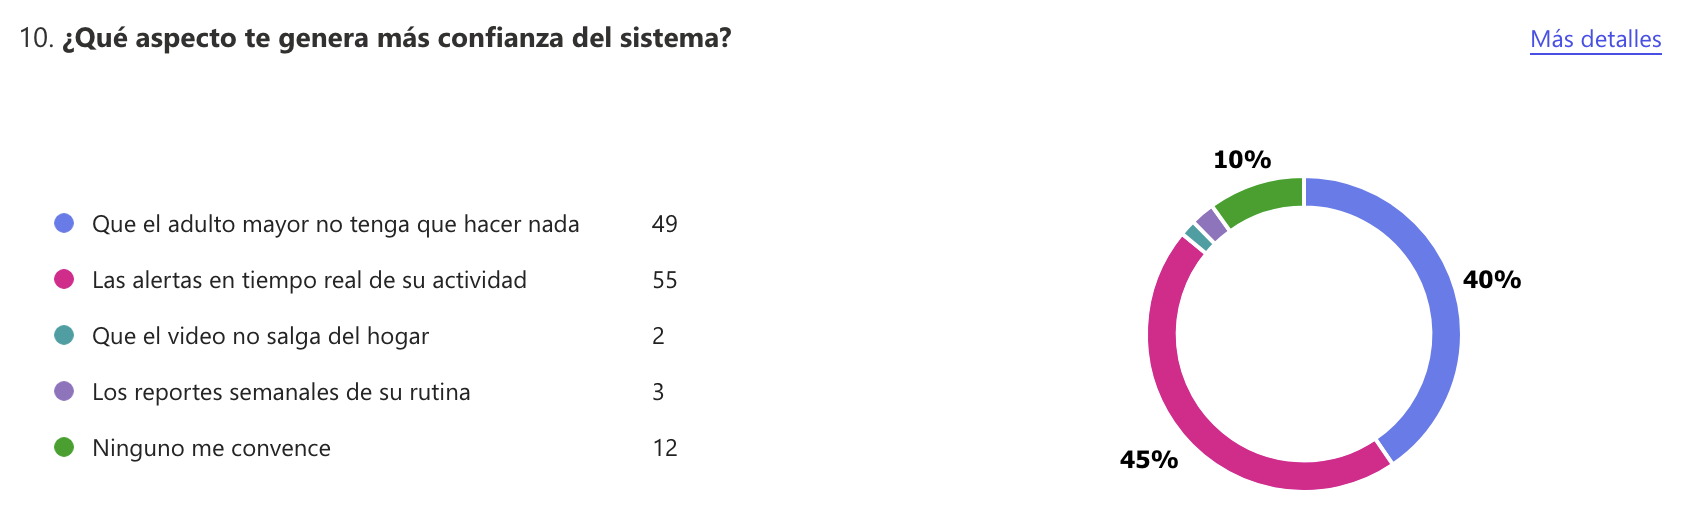
\includegraphics[width=0.85\textwidth]{Imagenes/Encuesta/Encuesta_Q10}
    \caption[Aspectos del sistema que generan más confianza en los cuidadores.]{Aspectos del sistema que generan más confianza en los cuidadores. Las alertas en tiempo real (45\,\%) y que el adulto mayor no deba operar ningún dispositivo (40\,\%) fueron los más valorados.
    \newline\footnotesize\textit{Fuente: Elaboración propia.}}
    \label{fig:encuesta_q10}
\end{figure}
